SSS 1a.
LINE

M = $<$ \{ $q_0, q_1, q_2$ \}, \{ I{ a, b, c }\}, \{ S{ A, B, C, Z }\}, \{ $\delta$ \}, $q_0$, Z, $q_2$ $>$ \\
BQ
$\delta$ ( $q_0$, a, S{Z} ) = ($q_1$, S{AZ}) \\
$\delta$ ( $q_0$, a, S{A} ) = ($q_1$, S{AA}) \\
$\delta$ ( $q_0$, b, S{Z} ) = ($q_1$, S{BZ}) \\
$\delta$ ( $q_0$, b, S{B} ) = ($q_2$, S{$\lambda$}) \\
$\delta$ ( $q_0$, b, S{A} ) = ($q_1$, S{BA}) \\
$\delta$ ( $q_1$, $\lambda$, S{Z} ) = ($q_3$, S{$\lambda$}) \\
$\delta$ ( $q_1$, c, S{A} ) = ($q_2$, S{$\lambda$}) \\
$\delta$ ( $q_1$, c, S{Z} ) = ($q_3$, S{CZ}) \\
$\delta$ ( $q_2$, c, S{C} ) = ($q_3$, S{CC}) \\
EQ
SSS 1b. 
LINE
M = $<$ \{ $q_0, q_1, q_2$ \}, \{ I{ a, b }\}, \{ S{ A, Z }\}, \{ $\delta$ \}, $q_0$, Z, $q_2$ $>$ \\
BQ
$\delta$ ( $q_0$, $\lambda$, S{Z} ) = ($q_2$, S{$\lambda$}) \\
$\delta$ ( $q_0$, a, S{Z} ) = ($q_0$, S{AA}), ($q_0$, S{AAA}) \\
$\delta$ ( $q_0$, a, S{A} ) = ($q_0$, S{AA}), ($q_0$, S{AAA})\\
$\delta$ ( $q_0$, b, S{A} ) = ($q_1$, S{$\lambda$}) \\
$\delta$ ( $q_1$, b, S{A} ) = ($q_1$, S{$\lambda$}) \\
$\delta$ ( $q_1$, $\lambda$, S{Z} ) = ($q_2$, S{$\lambda$})
EQ
SSS 1c.
M = $<$ \{ $q_0$ \}, \{ I{ a, b, c }\}, \{ S{ A, C, Z }\}, \{ $\delta$ \}, $q_0$, Z, emptyStack $>$ \\
BQ
$\delta$ ( $q_0$, a, S{Z} ) = ($q_0$, S{A}) \\
$\delta$ ( $q_0$, a, S{A} ) = ($q_0$, S{A}) \\
$\delta$ ( $q_0$, b, S{Z} ) = ($q_0$, S{A}) \\
$\delta$ ( $q_0$, b, S{A} ) = ($q_0$, S{A}) \\
$\delta$ ( $q_0$, a, S{C} ) = ($q_0$, S{$\lambda$}) \\
$\delta$ ( $q_0$, b, S{C} ) = ($q_0$, S{$\lambda$}) \\
$\delta$ ( $q_0$, c, S{Z} ) = ($q_0$, S{C}) \\
$\delta$ ( $q_0$, c, S{C} ) = ($q_0$, S{C}) \\
$\delta$ ( $q_0$, c, S{A} ) = ($q_0$, S{$\lambda$}) \\
EQ
Empty Stack
SSS 1d. 
Cannot be done as the language is not context-free. 
SSS 2. aa*b*a
BQ
$\delta$ ( $q_0$, a, S{Z} ) = ($q_0$, S{AZ}) \\
$\delta$ ( $q_0$, b, S{A} ) = ($q_0$, S{B}) \\
$\delta$ ( $q_0$, b, S{B} ) = ($q_0$, S{$\lambda$}), ($q_1$, S{B}) \\
$\delta$ ( $q_0$, $\lambda$, S{B} ) = ($q_0$, S{$\lambda$}) \\
$\delta$ ( $q_0$, a, S{A} ) = ($q_0$, S{$\lambda$}), ($q_1$, S{B}) \\
$\delta$ ( $q_1$, $\lambda$, S{Z} ) = ($q_0$, S{$\lambda$}) \\
EQ
SSS 3.
SSS 4.
\begin{center}
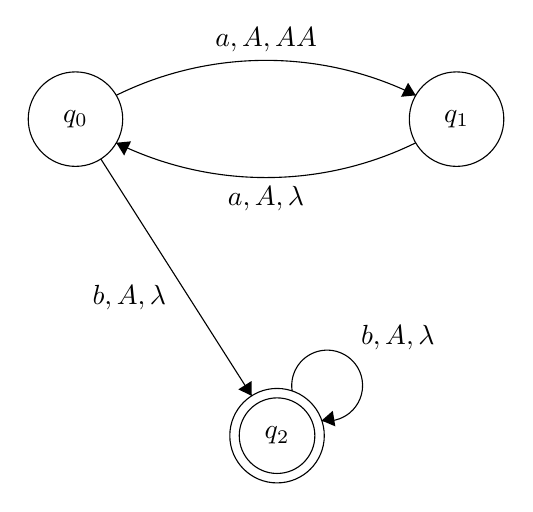
\begin{tikzpicture}[scale=0.2]
\tikzstyle{every node}+=[inner sep=0pt]
\draw [black] (25.1,-17.4) circle (3);
\draw (25.1,-17.4) node {$q_0$};
\draw [black] (49.3,-17.4) circle (3);
\draw (49.3,-17.4) node {$q_1$};
\draw [black] (37.9,-37.5) circle (3);
\draw (37.9,-37.5) node {$q_2$};
\draw [black] (37.9,-37.5) circle (2.4);
\draw [black] (38.86,-34.67) arc (189:-99:2.25);
\draw (43.2,-31.25) node [right] {$b,A,\lambda$};
\fill [black] (40.73,-36.54) -- (41.6,-36.91) -- (41.44,-35.92);
\draw [black] (26.71,-19.93) -- (36.29,-34.97);
\fill [black] (36.29,-34.97) -- (36.28,-34.03) -- (35.44,-34.56);
\draw (30.88,-28.76) node [left] {$b,A,\lambda$};
\draw [black] (27.688,-15.888) arc (116.29168:63.70832:21.474);
\fill [black] (46.71,-15.89) -- (46.22,-15.09) -- (45.77,-15.98);
\draw (37.2,-13.17) node [above] {$a,A,AA$};
\draw [black] (46.707,-18.904) arc (-63.86099:-116.13901:21.58);
\fill [black] (27.69,-18.9) -- (28.19,-19.71) -- (28.63,-18.81);
\draw (37.2,-21.61) node [below] {$a,A,\lambda$};
\end{tikzpicture}
\end{center}
BQ
$\delta$ ( $q_0$, a, S{Z} ) = ($q_1$, S{AA}) \\
$\delta$ ( $q_1$, a, S{A} ) = ($q_0$, S{$\lambda$}) \\
$\delta$ ( $q_0$, a, S{A} ) = ($q_1$, S{AA}) \\
$\delta$ ( $q_0$, b, S{A} ) = ($q_2$, S{$\lambda$}) \\
$\delta$ ( $q_2$, b, S{A} ) = ($q_2$, S{$\lambda$}) \\
EQ
SSS 5. 
(a+b+c)*$W$c$W^R$ is a deterministic context-free language while its reverse $W^R$c$W$(a+b+c)* is not.



